\section{Neutrino deep inelastic scattering (DIS)}
Il diagramma per la diffusione profondamente anelastica di neutrini da protone è
\begin{figure}[h!]
	\centering
	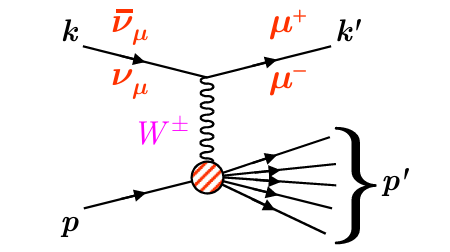
\includegraphics[width=0.6\textwidth]{Lezioni/Lezione 19/ala1.png}
	\label{fig:ala1}
\end{figure}
Si può parametrizzare l'elemento di matrice adronico per studiare interazioni profondamente anelastiche di neutrini (antineutrini). Un formalismo analogo a quello che si utilizza per lo scattering anelastico di elettroni. Per la sezione d'urto differenziale si trova (che dipende da due variabili non più da una sola)
$$
\frac{d\sigma}{dE_\mu^\prime d\Omega} \sim G^2 L^{\alpha\beta} W_{\alpha\beta}
$$
Il tensore $L^{\alpha\beta}$ è lo stesso di quello utilizzato nello studio delle interazioni leptoniche di neutrini (era $M^{\mu\nu}$ o $N^{\mu\nu}$). Il tensore $W^{\alpha\beta}$ si parametrizza con tre funzioni di struttura (funzioni di due variabili cinematiche)
$$
W^{\alpha\beta} = -g^{\alpha\beta}W_1 + \frac{1}{m_p^2}p^\alpha p^\beta W_2 - \frac{i}{2m_p^2}\varepsilon^{\alpha\beta\gamma\delta}p_\gamma q_\delta W_3
$$
Viene chiamata funzioni di struttura e non di forma perché quelle di forma sono quelle che entrano nell'elemento di matrice. Nel deep intelastic scatterin si utilizzano le variabili $Q^2=-q^2$ e $\nu=E_\nu-E_\mu$. Lo scattering non è elastico e una sola variabile non è sufficiente
$$
q^2 = (k - k^\prime)^2 = k^2 + k^{\prime 2} - 2k \cdot k^\prime \approx -2k \cdot k^\prime \approx -2E_\nu E_\mu (1 - \cos\theta)
$$
$$
q^2 = -4E_\nu E_\mu \sin^2\frac{\theta}{2} \qquad Q^2 = -q^2
$$
$$
\nu = E_\nu - E_\mu
$$
Inoltre, per la conservazione del $4-$momento, si ha
$$
p^\prime = p + q
$$
Sviluppando
$$
p^{\prime 2} = (p + q)^2 \quad \Rightarrow\quad M^{*2} \equiv p^{\prime 2} = m_p^2 + q^2 + 2q \cdot p
$$
$M^*$ massa invariante del sistema adronico
$$
M^{*2} = m_p^2 + q^2 + 2m_p\nu
$$
Per la sezione d'urto si trova ($W_i=W_i(q^2,\nu)$)
$$
\frac{d\sigma^{\nu,\bar{\nu}}}{dQ^2d\nu} = \frac{G^2}{2\pi} \frac{E_\mu}{E_\nu} \left( 2W_1 \sin^2\frac{\theta}{2} + W_2 \cos^2\frac{\theta}{2} \pm W_3 \frac{E_\nu + E_\mu}{m_p} \sin^2\frac{\theta}{2} \right)
$$
Qui quando noi abbiamo fatto uno scattering a due corpi quindi due particelle le variabili essenziali era una sola. Qui adesso abbiamo una pseudo particella di quadrimomento $p'$ ha la caratteristica che non ha un valore fissato come per le particelle reali perchè dipende dalla configurazione particolare. Questo significa che per descrivere questo processo serve una variabile in più.
Il segno $\pm$ della funzione $W_3$ è conseguenza della violazione di parità e vale $+$ per i neutrini e vale $-$ per gli antineutrini.
\section{Le variabili $x$ e $y$}
Si sostituiscono di solito le variabili $Q^2$ e $\nu=E_\nu-E'_\mu$ con le due variabili adimensionale $x$ e $y$ più adeguate per descrivere il limite di alto $Q$ (scaling)
$$
x = \frac{Q^2}{2m_p\nu} \qquad y = \frac{\nu}{E_\nu}
$$
Le variabili $x$ e $y$ possono essere espresse in funzioni di invarianti relativistici
$$
x = \frac{-q^2}{2p \cdot q} \qquad y = \frac{p \cdot q}{p \cdot k}
$$
Si può facilmente verificare che le espressioni precedenti si riducono alle espressioni originale nel sistema di laboratorio e si possono infine verificare le seguenti relazioni. Le regioni fisiche per le variabili $x$ e $y$ sono
$$
0 \le x \le 1 \qquad 0 \le y \le 1
$$
La variabile $y$ è legata all'angolo di diffusione nel centro di massa $\theta$
$$
1 - y = \frac{1}{2}(1 + \cos\theta) \qquad y = \frac{1}{2}(1 - \cos\theta)
$$
\section{Scaling di Bjorken}
La sezione d'urto per il DIS mostra un comportamento di tipo asintotico scoperto nel deep inelastic scattering $e-p$ a SLAC (Bjorken Scaling). Lui infatti interpretò tutti i comportamenti asintotici osservati. Fece le seguenti assunzioni:
\begin{itemize}
	\item Nel limite di grande $Q^2$
	\item nel limite di grande $\nu$
	\item per valori finiti del loro rapporto $x=\frac{Q^2}{2m_p\nu}=\frac{1}{\omega}$
\end{itemize}
Sotto queste condizioni le funzioni di struttura $W$ tendono a funzioni (universali) di $x$. In altre parole, la sezione d'urto dipende da una sola variabile cinematica come lo scattering elastico. Per il deep inelastic scattering di neutrini si ha
$$
m_p W_1(Q^2,\nu) \to F_1(x) \quad \nu W_2(Q^2,\nu) \to F_2(x) \quad \nu W_3(Q^2,\nu) \to F_3(x)
$$
$$
\frac{d\sigma^{\nu N}}{dxdy} = \frac{G^2 m_N E_\nu}{\pi} \left[ xy^2 F_1(x) + (1 - y)F_2(x) + xy\left( 1 - \frac{y}{2} \right) F_3(x) \right]
$$
\begin{figure}[h!]
	\centering
	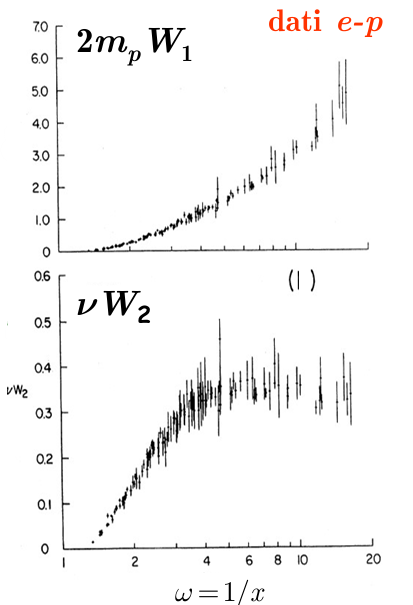
\includegraphics[width=0.3\textwidth]{Lezioni/Lezione 19/ala2.png}
	\label{fig:ala2}
\end{figure}
\section{Il modello a partoni}
Interpretiamo lo scattering profondamente anelastico con il modello a partoni. Il nucleo è composto da partoni ciascuno dei quali trasporta una frazione $\alpha$ del momento del nucleo. La probabilità che il partone $i-$esimo abbia una frazione $\alpha$ del momento totale del nucleone è dato da 
$$
\frac{dP}{d\alpha}=f_i(\alpha)
$$
\begin{figure}[h!]
	\centering
	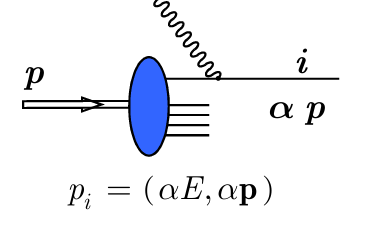
\includegraphics[width=0.3\textwidth]{Lezioni/Lezione 19/ala3.png}
	\label{fig:ala3}
\end{figure}
nella ipotesi che i partoni siano quarks utilizziamo le sezioni d'urto per lo scattering di neutrini o antineutrini. Per il momento, ci limitiamo alle interazioni di correnti cariche, quelle cioè che vedono la variazione di carica $\pm1$ per il fermione e che sono mediate dai bosoni vettoriali $W^{\pm}$, ad esempio:
\begin{figure}[h!]
	\centering
	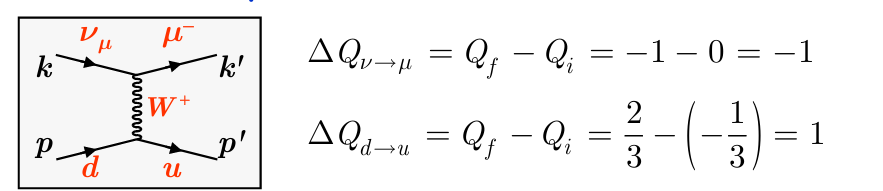
\includegraphics[width=0.6\textwidth]{Lezioni/Lezione 19/ala4.png}
	\label{fig:ala4}
\end{figure}
Nello studio delle interazioni leptoniche avevamo visto che la sezione d'urto era
$$
\frac{d\sigma}{d\Omega}=\frac{G^2s}{4\pi^2}|d_{i,j}|^2
$$
dove $d_{i,j}$ erano le matrici di rotazione per $J=1$.
\begin{figure}[h!]
	\centering
	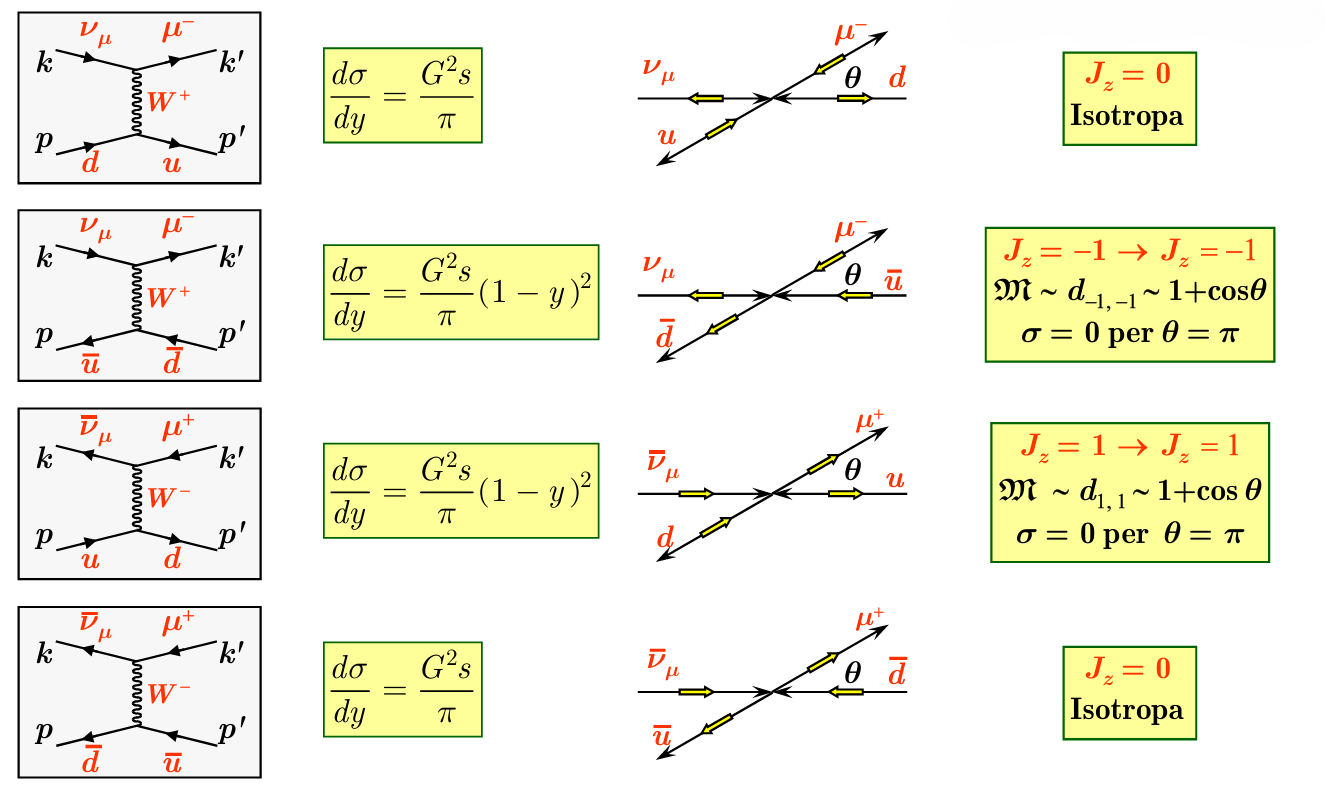
\includegraphics[width=0.6\textwidth]{Lezioni/Lezione 19/ala6.png}
	\label{fig:ala6}
\end{figure}
Quindi la sezione d'urto di nuetrino o di antineutrino è diverso. Con i neutrini vedo i quark $d$ o quark $\bar{u}$ che non dovrebbero esserci ma in piccole quantità in realtà ci sono. E stesso ragionamento per gli antineutrini. 
Utilizziamo il modello a partoni per interpretare i risultati dello scattering profondamente anelastico neutrino nucleone. La sezione d'urto è la somma incoerente delle sezioni d'urto dei singoli partoni pesate con le distribuzioni $f_i(x)$. La probabilità per il partone $i-esimo$ di avere una frazione $x$ del momento è $f_i(x)dx$ (si può dimostrare che $x$ coincide con la variabile introdotta precedentemente). 
\begin{figure}[h!]
	\centering
	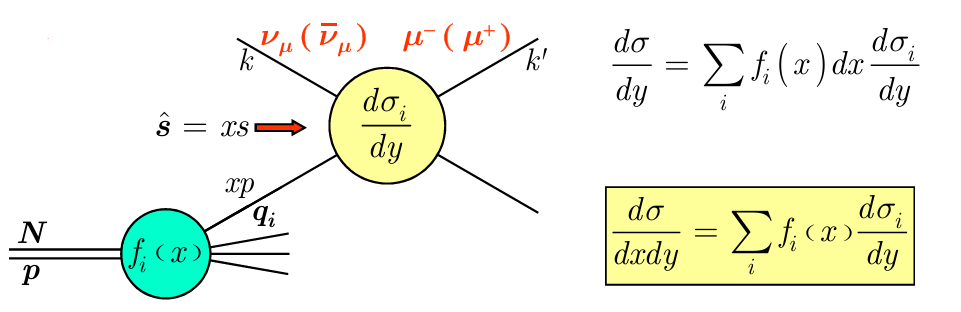
\includegraphics[width=0.6\textwidth]{Lezioni/Lezione 19/ala5.png}
	\label{fig:ala5}
\end{figure}
Se un partone trasporta una frazione $x$ del momento totale abbiamo che la variabile $\hat{s}$ per questo processo è (trascuriamo le masse)
$$
\hat{s} = (k + xp)^2 \approx 2xk \cdot p = xs
$$
La sezione d'urto del partone $i-$esimo viene calcolata a questa energia. Scriviamo l'espressione per la sezione d'urto $\nu-$protone. IL protone è composto da $2$ quark $u$ e un quark $d$ più eventuali quarks/anti-quarks del mare ($g\to q$ $\bar{q}\to g$). Il neutrino interagisce solo con i quark di valenza $d$ oppure con antiquark $\bar{u}$ del mare. La sezione d'urto $\nu-p$ pertanto è $(f_q(x)\to q(x))$
$$
\frac{d\sigma^{\nu p}}{dxdy} = d_p(x)\frac{d\sigma_{\nu d}}{dy} + \bar{u}_p(x)\frac{d\sigma_{\nu\bar{u}}}{dy}
$$
$$
\frac{d\sigma^{\nu p}}{dxdy} = \frac{G^2s}{\pi}x\left[ d_p(x) + \bar{u}_p(x)(1 - y)^2 \right]
$$
Analogamente la sezione d'urto $\bar{\nu}-p$ l'antineutrino interagisce solo con i quark di valenza $u$ oppure con antiquark $\bar{d}$ del mare
$$
\frac{d\sigma^{\bar{\nu} p}}{dxdy} = u_p(x)\frac{d\sigma_{\bar{\nu} u}}{dy} + \bar{d}_p(x)\frac{d\sigma_{\bar{\nu}\bar{d}}}{dy}
$$
$$
\frac{d\sigma^{\bar{\nu} p}}{dxdy} = \frac{G^2s}{\pi}x\left[ u_p(x)(1 - y)^2 + \bar{d}_p(x) \right]
$$
Scriviamo l'analoga espressione per la sezione d'urto $\nu-$neutrone. Il neutrono è composto da $2$ quark $d$ e un quark $u$ più eventuali quarks/antiquarks del mare ($g\to q$ $\bar{q}\to g$). IL neutrino interagisce solo con i quark di valenza $d$ oppure con antiquark $\bar{u}$ del mare. La sezione d'urto $\nu- n$ pertanto è
$$
\frac{d\sigma^{\nu n}}{dxdy} = \frac{G^2 s}{\pi} x \left[ d_n(x) + \bar{u}_n(x)(1 - y)^2 \right]
$$
Analogamente la sezione d'urto $\bar{\nu}-n$. L'antineutrino interagisce solo con i quark di valenza $u$ oppure con antiquark $\bar{d}$ del mare
$$
\frac{d\sigma^{\bar{\nu} n}}{dxdy} = \frac{G^2 s}{\pi} x \left[ u_n(x)(1 - y)^2 + \bar{d}_n(x) \right]
$$
Possiamo assumere che $n$ e $p$ siano un doppietto di isospin infatti sono sistemi speculari rispetto a scambio di $u$ e $d$
\begin{figure}[h!]
	\centering
	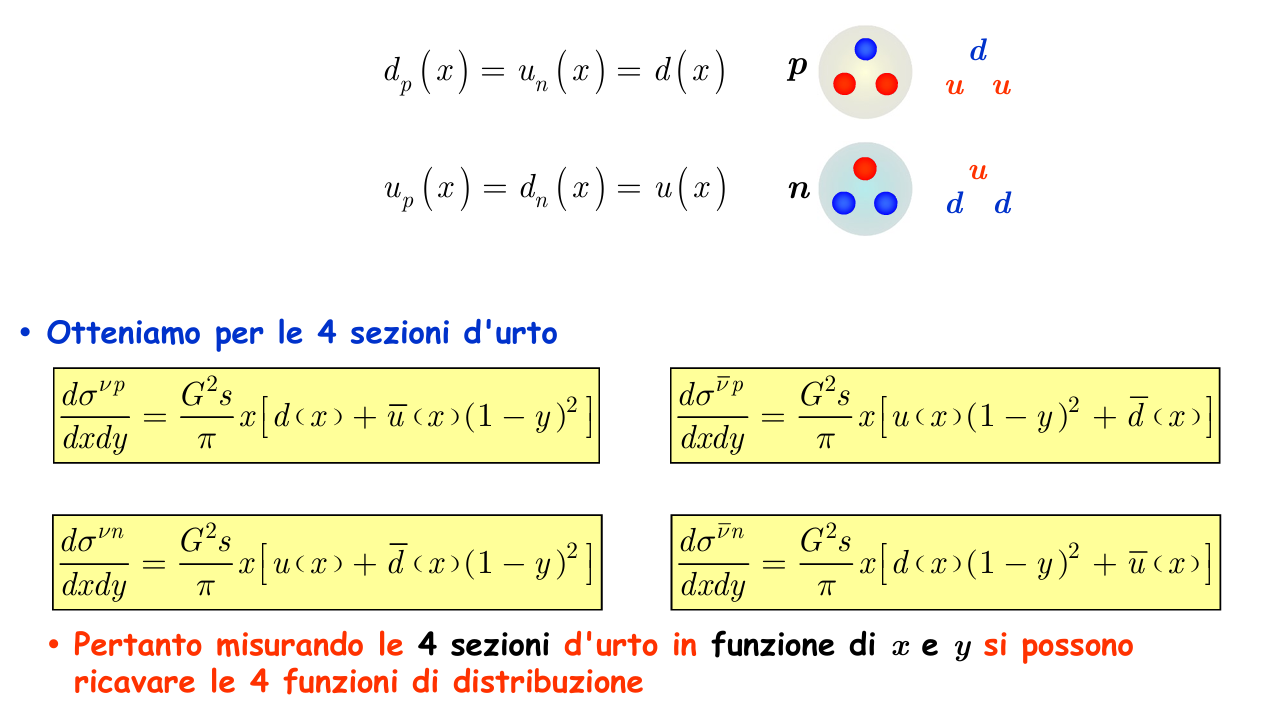
\includegraphics[width=0.8\textwidth]{Lezioni/Lezione 19/ala7.png}
	\label{fig:ala7}
\end{figure}
\section{La misura delle funzioni di distribuzione}
Da un punto di vista sperimentale occorre tenere conto che le sezioni d'urto di neutrini e antineutrini sono molto basse. Per aumentare la statistica occorre utilizzare materiali densi invece di idrogeno e deuterio. Si utilizzano come bersagli i cosiddetti materiali isoscalari i cui nuclei contengono lo stesso numero di neutroni e protoni. La sezione d'urto misurate sono in questo caso la media delle due sezioni d'urto trovate
$$
\frac{d\sigma^{\nu N}}{dxdy} \equiv \frac{1}{2}\left(\frac{d\sigma^{\nu p}}{dxdy} + \frac{d\sigma^{\nu n}}{dxdy}\right) = \frac{G^2 s}{2\pi} x \left[ u(x) + d(x) + (\bar{u}(x) + \bar{d}(x))(1-y)^2 \right]
$$
Dove
$$
q(x)=d(x)+u(x)
$$
Analogamente per le sezioni d'urto di antineutrini
$$
\frac{d\sigma^{\bar{\nu} N}}{dxdy} \equiv \frac{1}{2}\left(\frac{d\sigma^{\bar{\nu} p}}{dxdy} + \frac{d\sigma^{\bar{\nu} n}}{dxdy}\right) = \frac{G^2 s}{2\pi} x \left[ (u(x) + d(x))(1-y)^2 + \bar{u}(x) + \bar{d}(x) \right]
$$
Confrontiamo la formula generale dello scattering "deep inelastic" di neutrini con la formula appena ricavata
$$
\frac{d\sigma^{\nu N}}{dxdy} = \frac{G^2m_N E_\nu}{\pi}\left[ xy^2F_1 + (1 - y)F_2 + xy\left(1 - \frac{y}{2}\right)F_3 \right]
$$
$$
\frac{d\sigma^{\nu N}}{dxdy} = \frac{G^2s}{2\pi}x\left[ q(x) + \bar{q}(x)(1 - y)^2 \right]
$$
Uguagliando i coefficienti delle diverse potenze di $y$
$$
F_2 - (F_2 - xF_3)y + \frac{x}{2}(2F_1 - F_3)y^2 \quad x[q(x) + \bar{q}(x)] - 2x\bar{q}(x)y + x\bar{q}(x)y^2
$$
$$
\left\{\begin{aligned}F_2(x) &= xq(x) + x\bar{q}(x) \\ F_2(x) - xF_3(x) &= 2x\bar{q}(x) \\ 2F_1(x) - F_3(x) &= 2\bar{q}(x)\end{aligned}\right.
$$
$$
F_2(x) = xq(x) + x\bar{q}(x)
$$
Dal confronto delle soluzione per $F_2$ e $F_1$ si ritrova la relazione di Callan Gross
$$
2xF_1(x)=F_2(x)
$$
Questa relazione vale solo se sono fermioni quindi all'epoca era una scoperta del tipo "ok le particelle all'interno del protone e del neutrone sono fermioni e hanno spin $1/2$"
\section{Sezione d'urto differenziale}
\begin{figure}[h!]
	\centering
	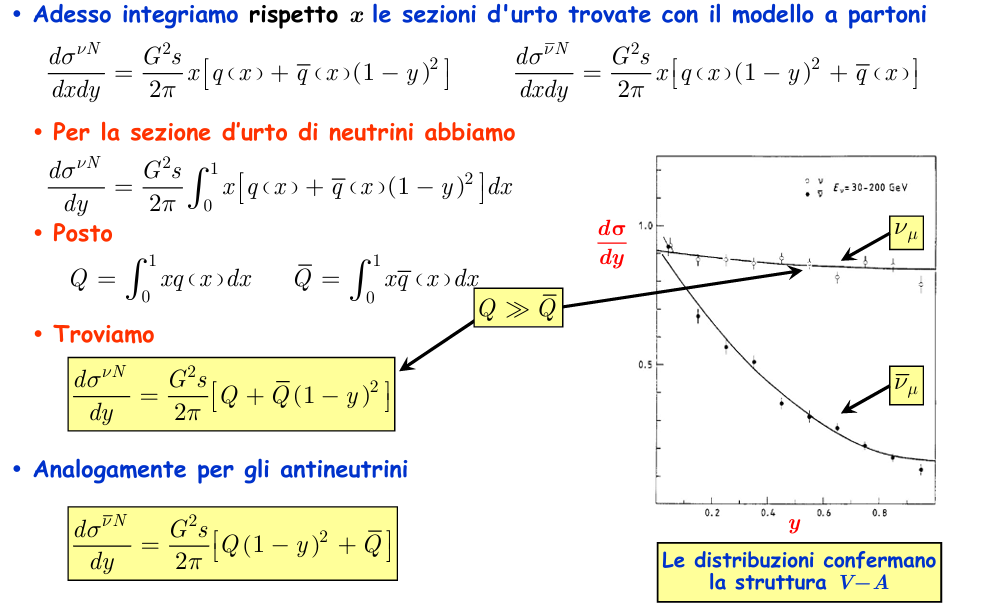
\includegraphics[width=0.8\textwidth]{Lezioni/Lezione 19/ala8.png}
	\label{fig:ala8}
\end{figure}
Quindi misuro una sezione d'urto in funzione di $y$ quindi dell'angolo. Guardando il grafico si vede che questa sezione d'urto o una sezione d'urto che è abbastanza isotropa anche se non troppo quindi vedo che ho più quark che anti-quark. Questi grafici dimostrano anche la struttura $V-A$ delle interazioni. In quanto vengono fatti i calcoli dalle correnti ecc ecc...
\section{Sezione d'urto totale}
\begin{figure}[h!]
	\centering
	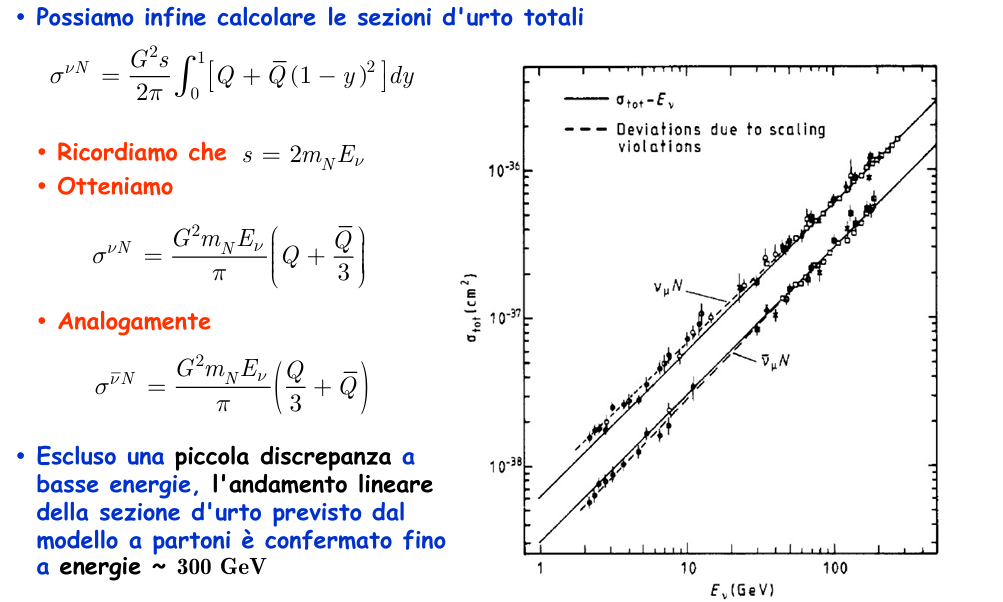
\includegraphics[width=0.8\textwidth]{Lezioni/Lezione 19/ala9.png}
	\label{fig:ala9}
\end{figure}
La sezione d'urto totale invece cosa ci fa capire? Due dipendenze (neutrino più alto) che avevamo già visto per i partoni. Queste curve sono abbastanza lineare. Queste approssimazioni di sezioni d'urto di capire se questi divergono al crescere dell'energia ma si vede che fino ad energie molto elevate funzionano bene. Studiamo il coefficiente della dipendenza lineare delle due sezioni d'urto
$$
\sigma^{\nu N} = \frac{G^2m_NE_\nu}{\pi}\left(Q + \frac{\bar{Q}}{3}\right) \quad \sigma^{\bar{\nu} N} = \frac{G^2m_NE_\nu}{\pi}\left(\frac{Q}{3} + \bar{Q}\right) 
$$
Preliminarmente, definiamo e calcoliamo il coefficiente $k$
$$
\frac{G^2s}{2\pi} = \frac{G^2m_NE_\nu}{\pi} \rightarrow \frac{G^2m_N}{\pi}(\hbar c)^2 E_\nu \equiv kE_\nu
$$
$$
k = \frac{\left(1.17 \times 10^{-5}\right)^2 \times 0.938 \times 0.389 \times 10^{-27}}{\pi} = 1.59 \times 10^{-38}
$$
Sperimentalmente si trova
$$
\left(\frac{\sigma_{Tot}}{E_\nu}\right)^{\nu N} = (0.64 \pm 0.03) \times 10^{-38} \text{ cm}^2\text{ GeV}^{-1}
$$
$$
\left(\frac{\sigma_{Tot}}{E_\nu}\right)^{\bar{\nu} N} = (0.31 \pm 0.02) \times 10^{-38} \text{ cm}^2\text{ GeV}^{-1}
$$
Si possono ricavare $(Q+\bar{Q})$ e $(Q-\bar{Q})$
\begin{figure}[h!]
	\centering
	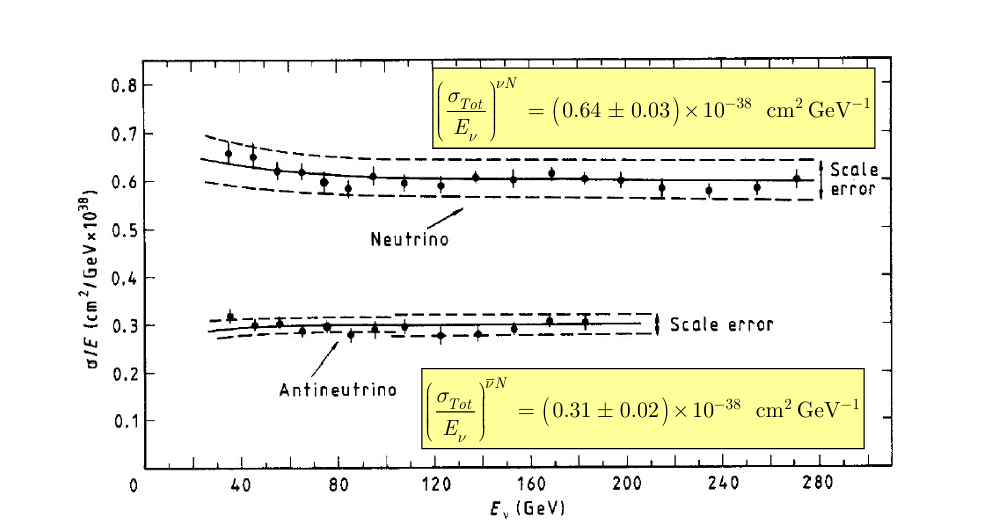
\includegraphics[width=0.6\textwidth]{Lezioni/Lezione 19/ala10.png}
	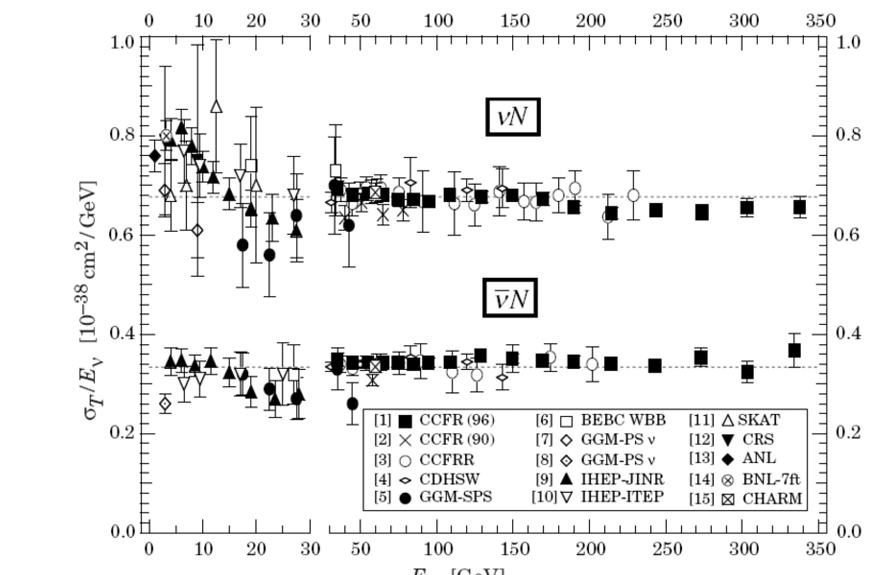
\includegraphics[width=0.6\textwidth]{Lezioni/Lezione 19/ala11.png}
	\label{fig:ala10}
\end{figure}
Negli anni sono state fatte questa misura in maniera più precisa con tantissimi esperimenti. Da queste misure escono fuori quei valori costanti. Sperimentalmente valori costanti e confrontando con le formule all'inizio della diapositiva recuperiamo $(Q+\bar{Q})$ e $(Q-\bar{Q})$.
\begin{figure}[h!]
	\centering
	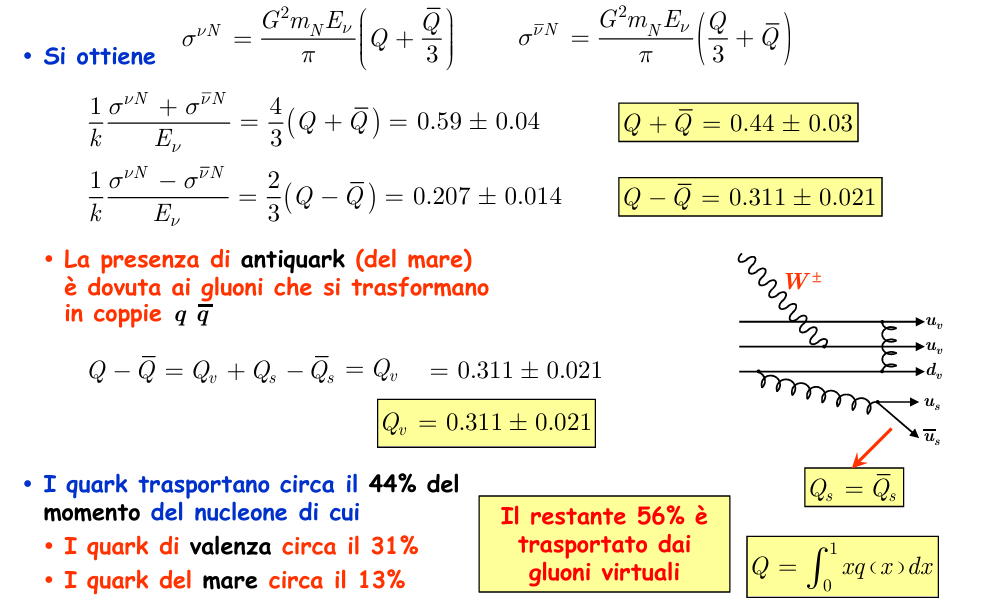
\includegraphics[width=0.8\textwidth]{Lezioni/Lezione 19/ala12.png}
	\label{fig:ala12}
\end{figure}
Dentro il nucleone ci sono gli antiquark questo perchè il $W$ può interagisre con i quark di valenza o con quelli che provengono dal mare che vengono prodotti dai gluoni. Il contributo dei quark e antiquark del mare non hanno nessun motivo per essere sbilanciati ma immagino che siano simmetrici. Se assumiamo questa cosa $Q-\bar{Q}$ mi da $Q_v$ quindi che frazione di momento totale quindi i quark trasportano solo il $30\%$ del momento. Il resto è traspostato dai gluoni! I gluonici sono e trasportano più della metà del momento ma non riesco a vederli con la mia sonda. 
\section{Le distribuzioni dei quark}
Le sezioni d'urto di neutrini e di anti-neutrini su neutroni e su protoni permettono di separare le distribuzioni dei quark up e down. Per misurare le sezioni d'urto su protone e neutrone occorre utilizzare bersagli di idrogeno e di deuterio. Purtroppo con questi materiali la massa del bersaglio è piccola. Esperimenti condotti tra la metà degli anni $'70$ e la metà degli anni $'80$. La statistica degli eventi fu limitata (circa $1000$ eventi per ogni esperiemenno). Le sezioni d'urto sono quindi integrate sulla variabile $y$. Le misure più accurate sono state fatte dagli esperimenti BEBC e CDHS "neutrinografia".
\section{Le distribuzioni $u(x)$ e $d(x)$}
\begin{figure}[h!]
	\centering
	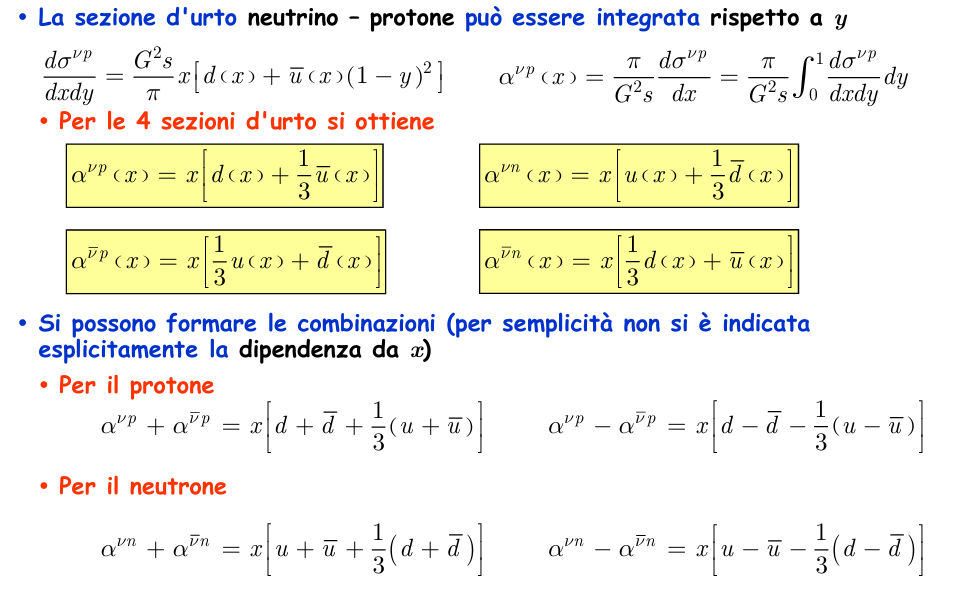
\includegraphics[width=0.8\textwidth]{Lezioni/Lezione 19/ala13.png}
	\label{fig:ala13}
\end{figure}
\begin{figure}[h!]
	\centering
	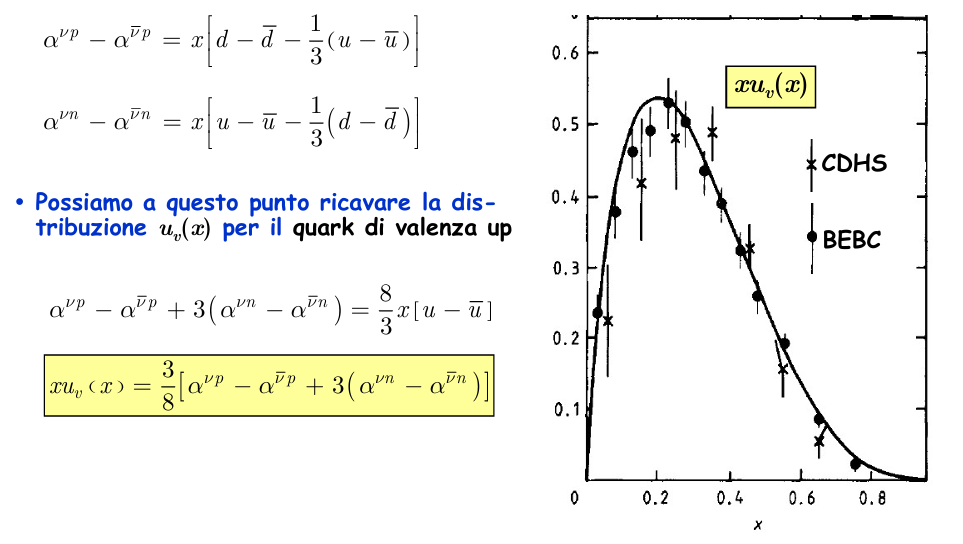
\includegraphics[width=0.5\textwidth]{Lezioni/Lezione 19/ala14.png}
	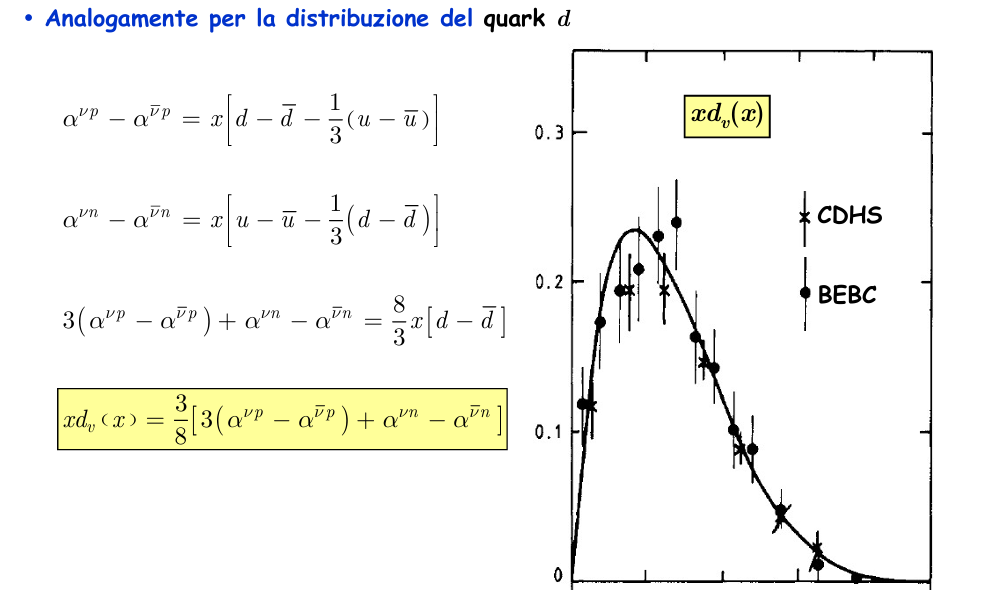
\includegraphics[width=0.5\textwidth]{Lezioni/Lezione 19/ala15.png}
	\label{fig:ala14}
\end{figure}
Queste sono le prime $PDF$ parton distribution functions.
\section{La scoperta delle correnti neutre}
Nel 1961 Glashow propose un modello per le interazioni deboli basato sul gruppo di gauge $SU(2)\times U(1)$. Nel 1967 Weinberg e Salam introdussero il meccanismo della rottura spontanea della simmetria per introdurre la massa. Nel 1971 't Hooft dimostrò che la teoria era rinormalizzabile. Il modello proposto prevedeva le correnti neutre tuttavia, nel corso degli anni 60, furono cercati, senza successo, decadimenti mediati da corrente neutra come ad esempio
$$
K^0\to\mu^+\mu^-
$$
Doveva essere anche un decadimento abbondante visto che l'energia disponibile è bella grande.
\begin{figure}[h!]
	\centering
	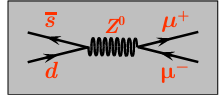
\includegraphics[width=0.3\textwidth]{Lezioni/Lezione 19/ala16.png}
	\label{fig:ala16}
\end{figure}
La corrente adronica genera una transizione da uno stato neutro ($K^0$) ad un altro stato neutro (il vuoto): $\Delta Q=0$. L'assenza del decadimento faceva ritenere che le correnti neutre o non esistessero o che avessero una intensità estremamente bassa. Nel 1970 Glashow, Iliopulos, Maiani: Meccanismo GIM per sopprimere le correnti neutre con cambiamento di flavour: FCNC. Le correnti neutre conservavano il flavour dei fermioni. Possono esistere anche se non esiste il decadimento sopracitato. Alla metà degli anni 60 A. Lagariggue, A. Rousset e P. Musset prepararono la proposta per la costruzione di una camera a bolle per la ricerca del Bosone Vettoriale Intermedio W mediante fasci di neutrini. La collaborazione era formata da diversi laboratori tra cui quelli di Milano. QUando il rivelatore entrò in funzione nel 1971, le priorità di ricerca erano:
\begin{itemize}
	\item Ricerca del BVI
	\item Ricerca di leptoni pesanti
	\item Deep inelastic scattering e violazione dello scaling
\end{itemize}
L'interesse dei fisici per il modello di Glashow, Weinberg, Salam aumentò notevolmente nel 1971 dopo il lavoro di 't Hooft sulla rinormalizzabilità della teoria. I teorici volevano cercare questo processo che non può avvenire con scambio di $W$ perchè le due famiglie sono distinte.
$$
\nu_\mu + e^- \rightarrow \nu_\mu + e^-
$$
Preferita degli sperimentali invece
$$
\nu_\mu + e^- \rightarrow \nu_\mu + e^-
$$
Il primo processo aveva il vantaggio della estrema chiarezza e basso fondo ma la sua sezione d'urto era molto piccola
$$
\sigma \sim G^2m_eE_\nu
$$
Il secondo aveva il vantaggio di una "alta" sezione d'urto ma fondo adronico e difficoltà di calcolo teorico.
Furono osservate diverse fotografie di eventi senza muone. Per poter affermare che si trattava di correnti neutre occorreva calcolare la proababilità di eventi di fondo: neutroni ad alta energia che interagiscono nella camera a bolle. Produzione di muoni molto lenti che non si vedono nella camera e muoni cosmici che fanno una interazione profondamente anelastica. Il problema principare era il fondo di neutroni, studiato mediante "gli eventi associati". L'idea era di dimostrare che le interazioni di neutrini sono distribuite uniformemente nel rivelatore e le interazioni di neutroni hanno un andamento esponenziale
$$
n(z)=n_0e^{-\rho_T\sigma_z}
$$
Mentre ferveva l'attività per valutare il background negli eventi di corrente neutra adronici fu trovato un evento candidato di interazione neutrino-elettrone mediato da corrente neutra. Il fondo per eventi di questo tipo era il decadimento di $\beta$ inverso. Quindi il problema del fondo di $\nu_e$ nel fascio di $\nu_\mu$
\begin{figure}[h!]
	\centering
	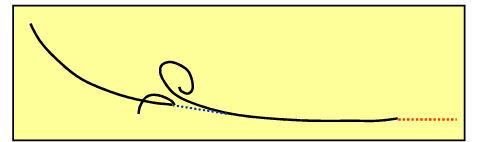
\includegraphics[width=0.3\textwidth]{Lezioni/Lezione 19/ala17.png}
	\label{fig:ala17}
\end{figure}